\documentclass{article} 
\usepackage[fleqn]{amsmath}
\usepackage{graphicx}
\usepackage{mathrsfs}
\usepackage{color}
\usepackage{amssymb}
\usepackage{amsfonts,amssymb}
\usepackage{algorithm}
\usepackage{algorithmic}
\usepackage{array}
\usepackage{latexsym}
\usepackage{hyperref}
\usepackage{amsthm}
%%%%% NEW MATH DEFINITIONS %%%%%

\usepackage{amsmath}\allowdisplaybreaks
\usepackage{amsfonts,bm}
\usepackage{amssymb}
\usepackage{dsfont}
\usepackage{amsthm}
\usepackage{algorithm}
\usepackage{algorithmic}

\theoremstyle{plain}
\newtheorem{theorem}{Theorem}%[section]
% \newtheorem{definition}{Definition}
% \newtheorem{example}{Example}
\newtheorem{lemma}{Lemma}
\newtheorem{assumption}{Assumption}
\newtheorem{remark}{Remark}
% \newtheorem{corollary}{Corollary}
\newtheorem{property}{Property}
\newtheorem{proposition}{Proposition}
\newtheorem{simplification}{Simplification}

\def\dif{\mathop{}\!\mathrm{d}}

\def\eps{{\varepsilon}}

\def\x{{\bf x}}
\def\X{{\bf X}}
\def\L{{\bf L}}



\def\bx{{\bar{x}}}
\def\hL{{\hat{L}}}
\def\hl{{\hat{\ell}}}

% Vectors
\def\vzero{{\bf{0}}}
\def\vone{{\bf{1}}}
\def\vmu{{\bm{\mu}}}
\def\vphi{{\bm{\phi}}}
\def\veta{{\bm{\eta}}}
\def\valpha{{\bm{\alpha}}}
\def\vbeta{{\bm{\beta}}}
\def\vtheta{{\bm{\theta}}}
\def\vnu{{\bm{\nu}}}
\def\vomega{{\bm{\omega}}}

\DeclareMathOperator{\KL}{KL}

% Graph
\def\cA{{\mathcal{A}}}
\def\cB{{\mathcal{B}}}
\def\cC{{\mathcal{C}}}
\def\cD{{\mathcal{D}}}
\def\cE{{\mathcal{E}}}
\def\cF{{\mathcal{F}}}
\def\cG{{\mathcal{G}}}
\def\cH{{\mathcal{H}}}
\def\cI{{\mathcal{I}}}
\def\cJ{{\mathcal{J}}}
\def\cK{{\mathcal{K}}}
\def\cL{{\mathcal{L}}}
\def\cM{{\mathcal{M}}}
\def\cN{{\mathcal{N}}}
\def\cO{{\mathcal{O}}}
\def\cP{{\mathcal{P}}}
\def\cQ{{\mathcal{Q}}}
\def\cR{{\mathcal{R}}}
\def\cS{{\mathcal{S}}}
\def\cT{{\mathcal{T}}}
\def\cU{{\mathcal{U}}}
\def\cV{{\mathcal{V}}}
\def\cW{{\mathcal{W}}}
\def\cX{{\mathcal{X}}}
\def\cY{{\mathcal{Y}}}
\def\cZ{{\mathcal{Z}}}

\def\scA{{\scriptscriptstyle\cA}}
\def\scD{{\scriptscriptstyle\cD}}
\def\scX{{\scriptscriptstyle\cX}}


% Sets
\def\BA{{\mathbb{A}}}
\def\BB{{\mathbb{B}}}
\def\BC{{\mathbb{C}}}
\def\BD{{\mathbb{D}}}
\def\BE{{\mathbb{E}}}
\def\BF{{\mathbb{F}}}
\def\BG{{\mathbb{G}}}
\def\BH{{\mathbb{H}}}
\def\BI{{\mathbb{I}}}
\def\BJ{{\mathbb{J}}}
\def\BK{{\mathbb{K}}}
\def\BL{{\mathbb{L}}}
\def\BM{{\mathbb{M}}}
\def\BN{{\mathbb{N}}}
\def\BO{{\mathbb{O}}}
\def\BP{{\mathbb{P}}}
\def\BQ{{\mathbb{Q}}}
\def\BR{{\mathbb{R}}}
\def\BS{{\mathbb{S}}}
\def\BT{{\mathbb{T}}}
\def\BU{{\mathbb{U}}}
\def\BV{{\mathbb{V}}}
\def\BW{{\mathbb{W}}}
\def\BX{{\mathbb{X}}}
\def\BY{{\mathbb{Y}}}
\def\BZ{{\mathbb{Z}}}

\def\xtij{x_{t,i,j}}
\def\ltij{\hl_{t,i,j}}

\newcommand{\Var}{\mathrm{Var}}
\newcommand{\standarderror}{\mathrm{SE}}
\newcommand{\Cov}{\mathrm{Cov}}
\newcommand{\Conv}{\mathrm{Conv}}
\newcommand{\rint}{\mathrm{int}}
\newcommand{\dom}{\mathrm{dom}}


\DeclareMathOperator*{\argmax}{arg\,max}
\DeclareMathOperator*{\argmin}{arg\,min}

\DeclareMathOperator{\sign}{sign}
\DeclareMathOperator{\Tr}{Tr}
\let\ab\allowbreak

\DeclareMathOperator{\diag}{diag}
\DeclareMathOperator{\spn}{span}
\DeclareMathOperator{\prox}{prox}






\newtheorem*{Solution}{Solution}
% \DeclareMathOperator*{\argmax}{arg\,max}

\newcommand{\mytextcolor}[1]{\textcolor{blue}{{}#1}}

\title{\normalsize
CS410: Artificial Intelligence 2021 Fall\\
Homework 4: Reinforcement
Learning \& Regression \\
Due date: 23:59:59 (GMT +08:00), December 3 2021}
\author{}
\date{}

\begin{document} 
\maketitle

\begin{enumerate}
    \item \textbf{TD Learning}.
    \begin{enumerate}
        \item     	Consider an MDP with states $A$, $B$, $C$, $D$, $E$, and $F$, where state $F$ is the terminal state. The agent will receive a reward $+1$ if it transits to the terminal state $F$ or receive a reward $0$ otherwise and the discount factor $\gamma=1$. Assume the current estimates of $V$ at time $t$ is $V_t (A)=0.2$,  $V_t (B)=0.4$,  $V_t (C)=0.6$,  $V_t (D)=0.8$,  $V_t (E)=1.0$, and $V_t (F)=0$. Further, suppose that our agent is at state $C$ at time $t$ and it will experience the following transitions shown in Figure 1 from time $t+1$ to time $t+7$. Use temporal difference (TD) learning with learning rate $\alpha=1/2$ to compute the new estimates of $V$ values of corresponding states each time the agent experiences a new transition. Finish this exercise by explicitly showing your computation process.
    
    
    $V_{t+1}(C)=\_\_$,
    $V_{t+2}(B)=\_\_$,
    $V_{t+3}(A)=\_\_$,
    $V_{t+4}(B)=\_\_$,\\
    $V_{t+5}(C)=\_\_$,
    $V_{t+6}(D)=\_\_$,
    $V_{t+7}(E)=\_\_$.
    
    	\begin{figure}[!htp]
    	    \centering
    	    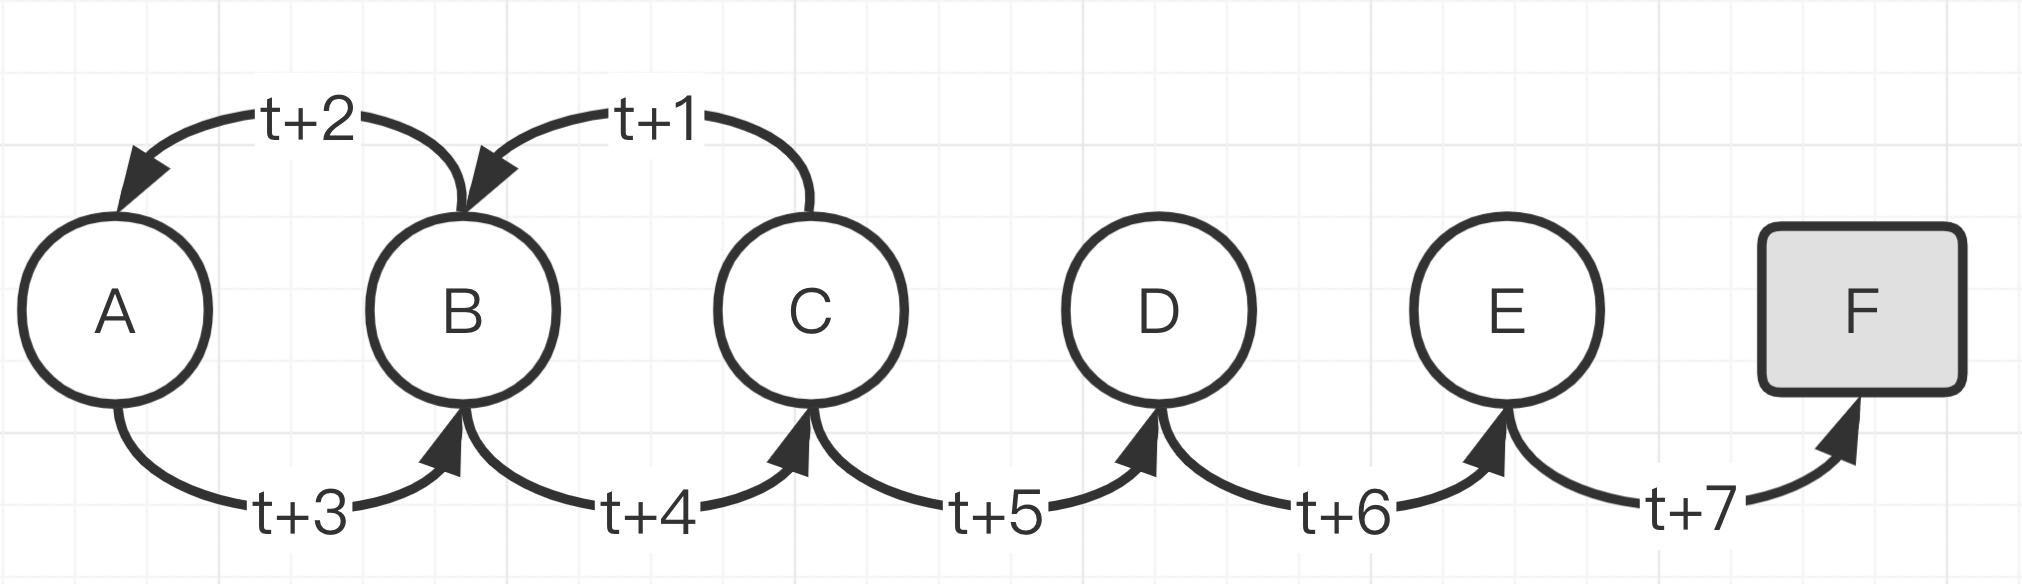
\includegraphics[width=12cm]{figs/fig1.png}
    	    \caption{Problem 1 (a).}
    	    \label{fig:p4}
    	\end{figure}
    	\begin{Solution}~\par
    	The update algorithm provides that
    	\begin{equation}
    	    \begin{aligned}
    	    sample=&R+\gamma\cdot V^\pi(s')\\
    	    V^\pi(s)\leftarrow V^\pi(s)+&\alpha\cdot(sample-V^\pi(s))
    	    \end{aligned}
    	\end{equation}
    	So following this rule, we have
    	\begin{equation}
    	    \begin{aligned}
    	    V_{t+1}(C)=0.6+0.5*(0.4-0.6)=0.5\\
    	    V_{t+2}(B)=0.4+0.5*(0.2-0.4)=0.3\\
    	    V_{t+3}(A)=0.2+0.5*(0.2-0.3)=0.25\\
    	    V_{t+4}(B)=0.3+0.5*(0.3-0.5)=0.4\\
    	    V_{t+5}(C)=0.5+0.5*(0.5-0.8)=0.65\\
    	    V_{t+6}(D)=0.8+0.5*(0.8-1.0)=0.9\\
    	    V_{t+7}(E)=1+0.5*(1-1)=1\\
    	    \end{aligned}
    	\end{equation}
    	Thus we get the answer
    	$V_{t+1}(C)=0.5,V_{t+2}(B)=0.3,V_{t+3}(A)=0.25,V_{t+4}(B)=0.4,V_{t+5}(C)=0.65,V_{t+6}(D)=0.9,V_{t+7}(E)=1$
    	\end{Solution}
    	\item 	Prove the statement in Lecture 7, Slide 38 that decreasing learning rate ($\alpha$) can give converging averages in TD learning.
    	
    	   % \mytextcolor{Update: 
    	   %  Recall the sequence $\{V_n\}$ with $V_n=(1-\alpha_n)V_{n-1}+\alpha_n x_n$ given in Lecture 7, Slide 38.
    	   %  Prove that $\{V_n\}$ converges by verifying that $\{V_n\}$ is a \href{https://en.wikipedia.org/wiki/Cauchy_sequence}{Cauchy sequence}
    	   % under the assumptions that (a) the learning rate $\alpha_t$ satisfies that $0<\alpha_t<1$ and $\lim_{t\to+\infty}\alpha_t=0$; and (b) discount factor $0<\gamma<1$, reward function $R$ is bounded, and $V_0(s)$ is bounded for all the state $s$ after $V_0$ is initialized. 
    	   % (Please ignore the old Problem 1 (b).)
    	   % }
    	    \mytextcolor{Update: 
    	     Prove the statement in Lecture 7, Slide 38 that decreasing learning rate ($\alpha$) can give converging averages in TD learning by verifying that the sequence $\{V_n\}$ with $V_n=(1-\alpha_n)V_{n-1}+\alpha_n x_n$ is a \href{https://en.wikipedia.org/wiki/Cauchy_sequence}{Cauchy sequence}
    	    under the assumption that $\forall n>0$, $\alpha_n=\frac{1}{n^2}$, $|x_n|\leq C_1$ and $|V_n|\leq C_2$ for some constants $C_1>0$ and $C_2>0$. )
    	    }
    	    \begin{Solution}~\par
    	    $V_n$ will converges$\Leftrightarrow$ $V_n$ is a Cauchy sequence, which means 
    	    \begin{equation}
    	        \forall~\epsilon>0,\exists~N\in\mathbb{N}, \forall~n>m>N, |V_{n}-V_{m}|<\epsilon.
    	    \end{equation}
    	    We know $x_n\le C_1,|V_n|\le C_2, \alpha_n=\frac{1}{n^2}$.\\
    	    So for given $\epsilon$, let $N=\lceil\frac{C_1+C_2}{\epsilon}\rceil$.
    	    Then we have
    	    \begin{equation}
    	        \begin{aligned}
    	            \forall~t,|V_t-V_{t+1}|=&|\alpha_{t+1}V_{t}+\alpha_{t+1}x_{t+1}|\le \frac{C_1+C_2}{(t+1)^2}\\
    	            \Rightarrow\forall n>m>N, &|V_n-V_m|=\sum_{k=m}^{n-1}|V_k-V_{k+1}|\\
    	        \le&(C_1+C_2)\cdot\sum_{k=m}^{n-1}\frac{1}{(k+1)^2}\\
    	        <&(C_1+C_2)\cdot\sum_{k=m}^{n-1}\frac{1}{(k+1)\cdot k}\\
    	        \le&(C_1+C_2)\cdot\sum_{k=m}^{n-1}\frac{1}{k}-\frac{1}{k+1}\\
    	        =&(C_1+C_2)\cdot(\frac{1}{m}-\frac{1}{n})\\
    	        \le&(C_1+C_2)\cdot\frac{1}{m}\\
    	        \le&(C_1+C_2)\cdot\frac{1}{N}\le\epsilon
    	        \end{aligned}
    	    \end{equation}
    	    \end{Solution}
    \end{enumerate}

    \item \textbf{Q-Learning.}
Recall the statement in Lecture 7, Slide 45 that Q-learning converges to optimal policy -- even if you're acting suboptimally. The task in this exercise is to prove this statement step by step. Let us first cover some preliminaries. Denote by $(X,d)$ the \href{https://en.wikipedia.org/wiki/Metric_space}{metric space}, where $X$ is a space and the metric $d:X\times X\to \BR$ is defined on pairs of elements in $X$. For example, let $X=\BR^n$ and
$d(x_1,x_2)=\|x_1-x_2\|_2$ for any $x_1, x_2 \in X$, where $\|\cdot\|_2$ denotes the \href{https://en.wikipedia.org/wiki/Norm_(mathematics)#Euclidean_norm}{2-norm}. Then
$d(x_1,x_2)$ denotes the Euclidean distance between $x_1$ and $x_2$. Let $H:X\to X $ be a mapping between 
the space $X$ and itself. If there exists some $0<L<1$, s.t. $\forall x,y\in X$, $d(H(x),H(y))\leq L\cdot
d(x,y)$, then the mapping $H$ is defined as a contradiction mapping. If there exists a point $x\in X$
s.t. $H(x)=x$, then $x$ is defined as the fixed-point of mapping $H$. If $H$ is a contradiction mapping,
then it could be shown that $H$ admits a unique fixed-point $x^\ast$ in $X$. 
\begin{enumerate}
    \item 	Recall that the optimal $Q^\ast$ satisfies the optimal Bellman equation
    \begin{align*}
        Q^{*}(s, a)=\sum_{s^{\prime}} T\left(s, a, s^{\prime}\right)\left[R\left(s, a, s^{\prime}\right)+\gamma \max _{a^{\prime}} Q^{*}\left(s^{\prime}, a^{\prime}\right)\right]\,.
    \end{align*}
    If we treat $X$ as the space of $Q$ functions (i.e., each element $q$ in $X$ is a $Q$ function, which further specifies a $Q$ value $q(s,a)$ for a given state-action pair $(s,a)$), and treat $H$ as
    \begin{align*}
        H:q(s,a)\mapsto \sum_{s^{\prime}} T\left(s, a, s^{\prime}\right)\left[R\left(s, a, s^{\prime}\right)+\gamma\max_{a^\prime} q\left(s^{\prime},a^\prime\right)\right]\,.
    \end{align*}
    Then it is clear that $Q^\ast$ is the fixed-point of $H$ since 
    $Q^\ast=H(Q^\ast)$.
    Assume the discount factor $0<\gamma<1$. Prove that $H$ is a contradiction mapping with respect to the metric
    \begin{align*}
        d(q_1,q_2)=||q_1-q_2||_{\infty}=\max_{s,a}|q_1(s,a)-q_2(s,a)|
    \end{align*}
    for any two $Q$ functions $q_1$ and $q_2$, where $\|\cdot\|_\infty$ is the \href{https://en.wikipedia.org/wiki/Norm_(mathematics)#Maximum_norm_(special_case_of:_infinity_norm,_uniform_norm,_or_supremum_norm)}{maximum norm}  (i.e., prove that
    $\|H(q_1)-H(q_2)\|_{\infty}\leq \gamma\|q_1-q_2\|_{\infty}$
    for any two $Q$ functions $q_1$ and $q_2$).
    \begin{Solution}~\par
    First, since the definition of $T$, we have
    \begin{equation}
        \sum_{s^{\prime}} T(s, a, s^{\prime})=1
    \end{equation}
    Then we have 
    \begin{equation}
        \begin{aligned}
        &\|H(q_1)-H(q_2)\|_{\infty}=\max_{s,a}\left|q_1(s,a)-q_2(s,a)\right|\\
        =&\max_{s,a}|\sum_{s^{\prime}} T\left(s, a, s^{\prime}\right)\left[R\left(s, a, s^{\prime}\right)+\gamma\max_{a^\prime} q_1\left(s^{\prime},a^\prime\right)\right]\\-&\sum_{s^{\prime}} T\left(s, a, s^{\prime}\right)\left[R\left(s, a, s^{\prime}\right)+\gamma\max_{a^\prime} q_2\left(s^{\prime},a^\prime\right)\right]|\\
        =&\max_{s,a}|\sum_{s^{\prime}} T\left(s, a, s^{\prime}\right)\left[R\left(s, a, s^{\prime}\right)+\gamma\max_{a^\prime} q_1\left(s^{\prime},a^\prime\right)\right.\\&\left.-R\left(s, a, s^{\prime}\right)-\gamma\max_{a^\prime} q_2\left(s^{\prime},a^\prime\right)\right]|\\
        =&\max_{s,a}|\sum_{s^{\prime}} T\left(s, a, s^{\prime}\right)\left[\gamma\max_{a^\prime} q_1\left(s^{\prime},a^\prime\right)-\gamma\max_{a^\prime} q_2\left(s^{\prime},a^\prime\right)\right]|\\
        =&\gamma\cdot\max_{s,a}|\sum_{s^{\prime}} T\left(s, a, s^{\prime}\right)\left[\max_{a^\prime} q_1\left(s^{\prime},a^\prime\right)-\max_{a^\prime} q_2\left(s^{\prime},a^\prime\right)\right]|\\
        \le&\gamma\cdot\max_{s,a}|\sum_{s^{\prime}} T\left(s, a, s^{\prime}\right)\|q_1-q_2|_{\infty}|\\
        \le&\gamma\|q_1-q_2|_{\infty}\cdot\max_{s,a}\sum_{s^{\prime}} T\left(s, a, s^{\prime}\right)\\
        =&\gamma\|q_1-q_2|_{\infty}
        \end{aligned}
    \end{equation}
    \end{Solution}
    \item	Consider an finite MDP  $(\cS,\cA,T,R, \gamma)$ with finite state space $\cS$ and finite action space $\cA$. Assume the reward function $R$ is bounded and deterministic and $0<\gamma<1$. Recall that Q-learning updates $Q$ function as
    \begin{align*}
        Q_{t+1}(s_t,a_t)&=Q_t(s_t,a_t)-\alpha_t(Q_t(s_t,a_t)-\text{sample}_t)\\
        &=(1-\alpha_t)Q_t(s_t,a_t)+\alpha_t\cdot\text{sample}_t\,,
    \end{align*}
    where $\text{sample}_t=R(s_t,a_t,s^\prime)+\gamma\max_{a^\prime}Q_{t}(s^\prime,a^\prime)$, $0\leq \alpha_t\leq 1$ is the learning rate at time $t$, and $\{s_t\}$ is the sequence of states obtained
    following policy $\pi$, which satisfies 
    $\mathbb{P}_{\pi}\left[A_{t}=a \mid S_{t}=s\right]>0$ for all
    state-action pairs $(s,a)$. Prove that Q-learning converges to $Q^\ast$ if $\sum_{t} \alpha_{t}=\infty$ and $\sum_{t} \alpha^2_{t}<\infty$. First construct a sequence $\Delta_{t+1}(s,a)=Q_t(s,a)-Q^\ast(s,a)$ using the update rule of Q-learning and $Q^\ast$. Then verify that the three assumptions in Lemma 1 hold. Finally apply Lemma 1 to finish this exercise. 
    
    \mytextcolor{Update: Further assume that $Q^\ast(s,a)$ is bounded for all the state-action pair $(s,a)$, and $Q_t(s,a)$ is bounded for all the state-action pair $(s,a)$, $\forall t>0$.}
    \begin{lemma}
        The random process $\{\Delta_t\}$ taking values in $\BR$ and defined as
        \begin{align*}
            \Delta_{t+1}(x)=\left(1-\alpha_{t}\right) \Delta_{t}(x)+\alpha_{t} F_{t}(x)
        \end{align*}
        converges to $0$ under the following assumptions:
        \begin{itemize}
            \item $0\leq\alpha_{t}\leq1$, $\sum_{t} \alpha_{t}=\infty$ and $\sum_{t} \alpha^2_{t}<\infty$;
            \item $\left\|\mathbb{E}\left[F_{t} \mid \mathcal{F}_{t}\right]\right\|_{\infty} \leq \gamma\left\|\Delta_{t}\right\|_{\infty}$ with $\gamma<1$, where $\cF_t=\{\Delta_t,\Delta_{t-1},\ldots,\Delta_1,F_{t-1},\ldots,F_1\}$ stands for the past information at time $t$, and $\mathbb{E}\left[F_{t} \mid \mathcal{F}_{t}\right]$ denotes the \href{https://en.wikipedia.org/wiki/Conditional_expectation}{conditional expectation} of $F_{t}$ given $\mathcal{F}_{t}$;
            \item $\BV\left[F_{t}(x) \mid \mathcal{F}_{t}\right] \leq C\left(1+\left\|\Delta_{t}\right\|_{\infty}\right)^2$ for some constant $C>0$, where $\BV\left[F_{t}(x) \mid \mathcal{F}_{t}\right]$ denotes the \href{https://en.wikipedia.org/wiki/Conditional_variance}{conditional variance} of $F_{t}(x)$ given $\mathcal{F}_{t}$.
        \end{itemize}
    \end{lemma}
    \begin{Solution}~\par
    Firstly, construct $\Delta_{t+1}(s,a)$ that
    \begin{equation}
    \begin{aligned}
        &\Delta_{t+1}(s,a)=Q_t(s,a)-Q^\ast(s,a)\\
        =&(1-\alpha_t)\cdot Q_t(s,a)+\alpha_t\left[R\left(s, a, s^{\prime}\right)+\gamma\max_{a^\prime} q\left(s^{\prime},a^{\prime}\right)\right]\\
        -&(1-\alpha_t)\cdot Q^\ast(s,a)-\alpha_t\cdot Q^\ast(s,a)\\
        =&(1-\alpha_t)\cdot\left[Q_t(s,a)-Q^\ast(s,a)\right]\\+&\alpha_t\cdot \left[R\left(s, a, s^{\prime}\right)+\gamma\max_{a^\prime} Q_t\left(s^{\prime},a^{\prime}\right)-Q^\ast(s,a)\right]\\
        :=&(1-\alpha_t)\cdot\Delta_{t}(s,a)+F_t(s,a)
    \end{aligned}
    \end{equation}
    And for the \textbf{Lemma 1}:
    \begin{enumerate}
        \item We set $\sum_{t}\alpha_t=\infty,\sum_t\alpha_t^2<\infty$
        \item From above we know $H$ is a contradiction mapping and $Q^\ast$ is the fixed-pointed, so we have
        \begin{equation}
            \begin{aligned}
            \left\|\mathbb{E}\left[F_{t} \mid \mathcal{F}_{t}\right]\right\|_{\infty}&=\max_{s,a}|\sum_{s^{\prime}} T\left(s, a, s^{\prime}\right)\left[R\left(s, a, s^{\prime}\right)+\gamma \max _{a^{\prime}} Q^{*}\left(s^{\prime}, a^{\prime}\right)\right]-Q^\ast(s,a)|\\
            &=\|H(Q_t(s,a))-H(Q^\ast(s,a))\|\\
            &\leq \gamma\|Q_t(s,a)-Q^\ast(s,a)\|\\
            &= \gamma\left\|\Delta_{t}\right\|_{\infty}
            \end{aligned}
        \end{equation}
        \item For the variance, and $F_t$ is independent tp $Q^\ast$, we have
        \begin{equation}
            \begin{aligned}
            \mathbb{V}\left[F_t(s,a)\right]&=\mathbb{V}\left[F_t(s,a)+Q^\ast(s,a)\right]-\mathbb{V}\left[Q^\ast(s,a)\right]\\
            &=\mathbb{V}\left[R(s,a,s')+\gamma\max_{a'}Q_t(s',a')\right]-0\\
            &=\mathbb{E}\left[R(s,a,s')+\gamma\max_{a'}Q_t(s',a')\right]^2-\mathbb{E}^2\left[R(s,a,s')+\gamma\max_{a'}Q_t(s',a')\right]
            \end{aligned}
        \end{equation}
        Since for the conditional variance, and we know $R,Q_t$ are both bounded, assume the bound is $R_{max},Q_{max}$, \\so $\exists C=(R_{max}+\gamma\cdot Q_{max})^2$ that
        \begin{equation}
            \begin{aligned}
            \mathbb{V}\left[F_t|\mathcal{F}_{t}\right]=&\mathbb{E}\left[R(s,a,s')+\gamma\max_{a'}Q_t(s',a')|\mathcal{F}_{t}\right]^2-\mathbb{E}^2\left[R(s,a,s')+\gamma\max_{a'}Q_t(s',a')|\mathcal{F}_{t}\right]\\
            \le&\mathbb{E}\left[R(s,a,s')+\gamma\max_{a'}Q_t(s',a')|\mathcal{F}_{t}\right]^2\le C
            \end{aligned}
        \end{equation}
    \end{enumerate}
    Finally, based on the \textbf{Lemma 1}, we know $\Delta_t\rightarrow0$. \\Since $\mathbb{P}_{\pi}\left[A_{t}=a \mid S_{t}=s\right]>0$, we can conclude $Q_t(s,a)\rightarrow Q^\ast(s,a)$ for all state-action pairs.
    \end{Solution}
\end{enumerate}
\item \textbf{Regression.}
Recall the exercise in Lecture 8, Slide 21. Some economists say that the impact of GDP in `current year' will have an effect on vehicle sales `next year'. So whichever year GDP was less, the coming year sales were lower, and when GDP increased the next year vehicle sales also increased. Let's have the equation as 
$y=\theta_0+\theta_1 x$
, where $y = \text{number of vehicles sold in the year}$ and $x = \text{GDP of the prior year}$. We need to find $\theta_0$ and $\theta_1$. Here is the data between 2011 and 2016.
    	\begin{figure}[!htp]
    	    \centering
    	    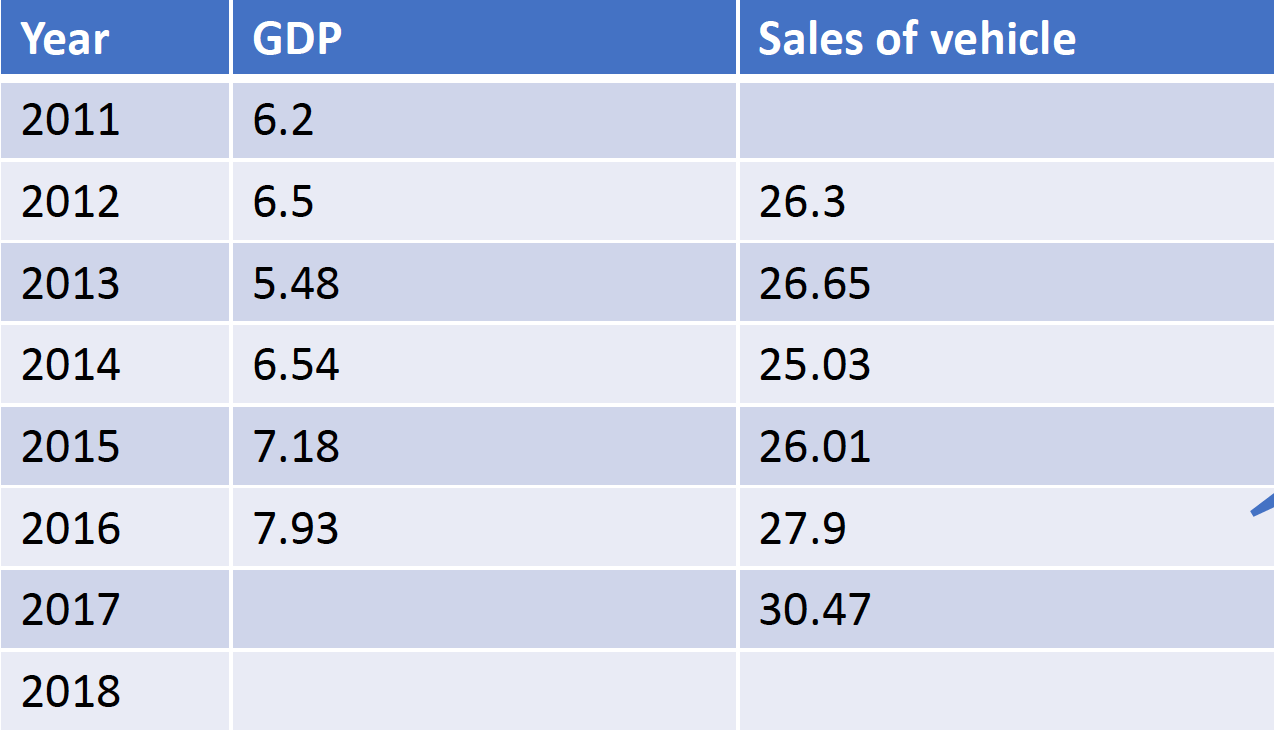
\includegraphics[width=12cm]{figs/fig2.png}
    	    \caption{Problem 3.}
    	    \label{fig:p4}
    	\end{figure}
    	\begin{enumerate}
    	    \item What is the normal equation?
    	    \begin{Solution}
    	    The formula for normal equation is
    	    \begin{equation}
    	        \mathbf{X}^T\mathbf{X}\theta=\mathbf{X}^Ty
    	    \end{equation}
    	    In this problem, we have
    	    \begin{equation}
    	  \mathbf{X}=\left[\begin{aligned}
    	  1~~~~6.2\\
    	  1~~~~6.5\\
    	  1~~~~5.48\\
    	  1~~~~6.54\\
    	  1~~~~7.18\\
    	  1~~~~7.93
    	  \end{aligned}\right],~y=\left[\begin{aligned}
    	  26.3\\26.65\\25.03\\26.01\\27.9\\30.47
    	  \end{aligned}\right]
    	    \end{equation}
    	    Then we have
    	    \begin{equation}
    	  \mathbf{X}^T\mathbf{X}=\left[\begin{aligned}
    	  6.0~~~~39.83~\\
    	  39.83~~~267.93
    	  \end{aligned}\right],~\mathbf{X}^Ty=\left[\begin{aligned}
    	  162.36\\1085.5
    	  \end{aligned}\right]
    	    \end{equation}
    	    So the solution of the equation is
    	    \begin{equation}
    	  \theta=\left[\begin{aligned}
    	  12.56\\2.18~
    	  \end{aligned}\right]\Rightarrow~y=12.56+2.18x
    	    \end{equation}
    	    \end{Solution}
    	    \item Suppose the GDP increasement in 2017 is 7\%, how many vehicles will be sold in 2018?
    	    \begin{Solution}
    	    This time, we get $x=7$, then we have $y=12.56+2.18\times7=27.82$
    	    \end{Solution}
    	\end{enumerate}
\end{enumerate}

\end{document} 
